\documentclass{standalone}
\usepackage{tikz}
\usetikzlibrary{patterns, positioning}


\begin{document}
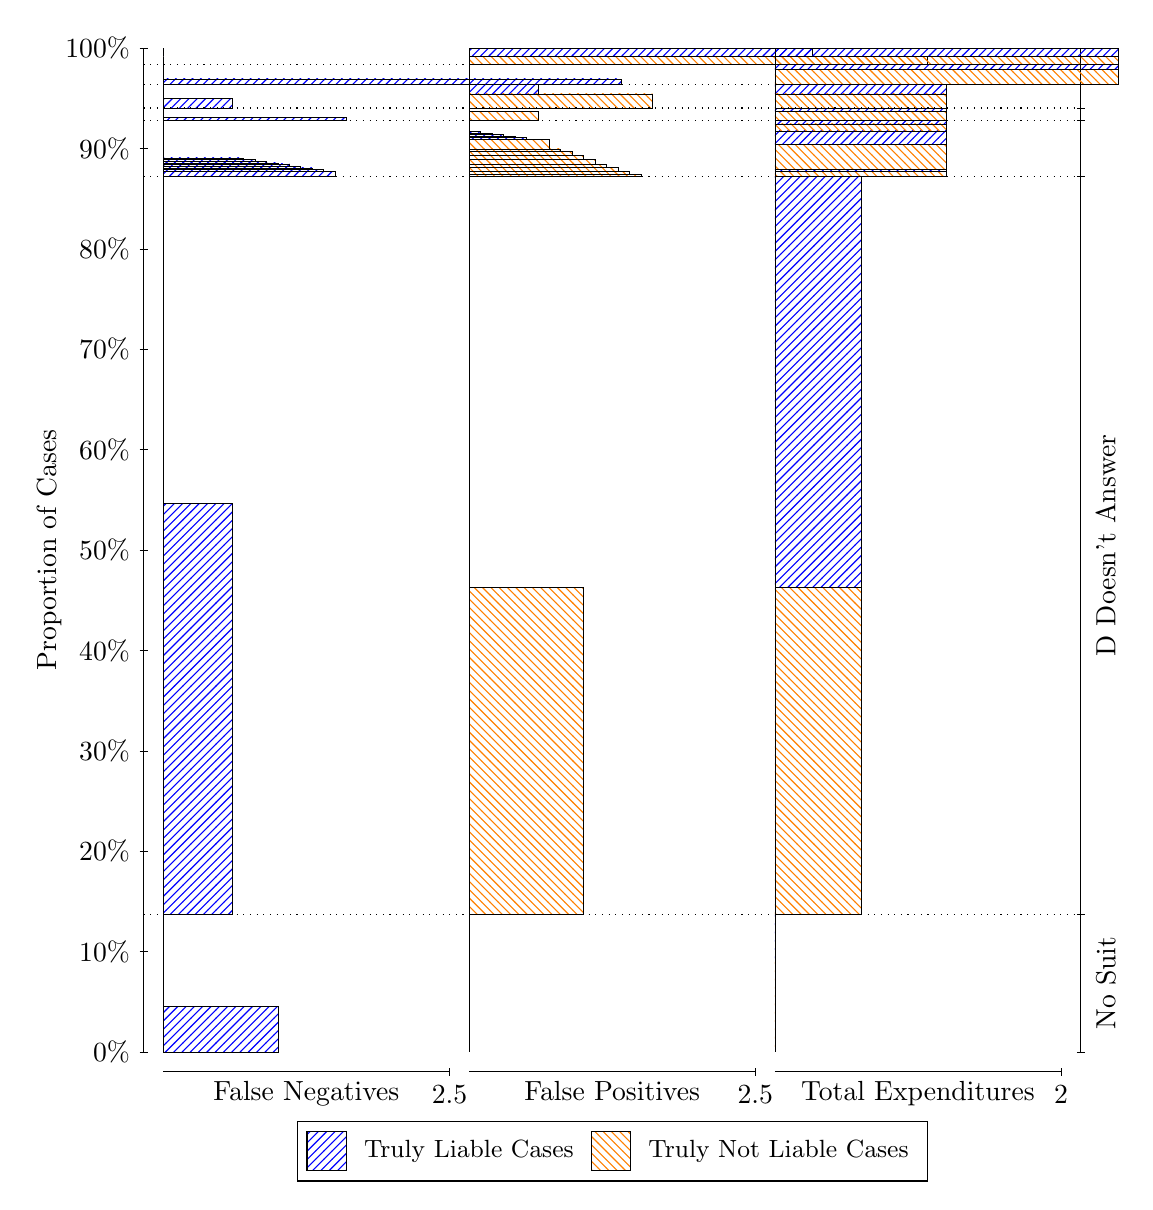
\begin{tikzpicture}
\draw[black, very thin] (1.5,1.75) -- (1.5,14.5);
\node[rotate=90, text=black, anchor=center] at (0.3, 8.125) {Proportion of Cases};
\draw[black, very thin] (1.45,1.75) -- (1.55,1.75);
\node[text=black, anchor=east] at (1.45, 1.75) {0\%};
\draw[black, very thin] (1.45,3.025) -- (1.55,3.025);
\node[text=black, anchor=east] at (1.45, 3.025) {10\%};
\draw[black, very thin] (1.45,4.3) -- (1.55,4.3);
\node[text=black, anchor=east] at (1.45, 4.3) {20\%};
\draw[black, very thin] (1.45,5.575) -- (1.55,5.575);
\node[text=black, anchor=east] at (1.45, 5.575) {30\%};
\draw[black, very thin] (1.45,6.85) -- (1.55,6.85);
\node[text=black, anchor=east] at (1.45, 6.85) {40\%};
\draw[black, very thin] (1.45,8.125) -- (1.55,8.125);
\node[text=black, anchor=east] at (1.45, 8.125) {50\%};
\draw[black, very thin] (1.45,9.4) -- (1.55,9.4);
\node[text=black, anchor=east] at (1.45, 9.4) {60\%};
\draw[black, very thin] (1.45,10.675) -- (1.55,10.675);
\node[text=black, anchor=east] at (1.45, 10.675) {70\%};
\draw[black, very thin] (1.45,11.95) -- (1.55,11.95);
\node[text=black, anchor=east] at (1.45, 11.95) {80\%};
\draw[black, very thin] (1.45,13.225) -- (1.55,13.225);
\node[text=black, anchor=east] at (1.45, 13.225) {90\%};
\draw[black, very thin] (1.45,14.5) -- (1.55,14.5);
\node[text=black, anchor=east] at (1.45, 14.5) {100\%};

\draw[black, very thin] (13.4,1.75) -- (13.4,14.5);
\draw[black, very thin] (13.35,1.75) -- (13.45,1.75);
\node[anchor=west] at (13.35, 1.75) {};
\draw[black, very thin] (13.35,3.4972) -- (13.45,3.4972);
\node[anchor=west] at (13.35, 3.4972) {};
\draw[black, very thin] (13.35,12.868) -- (13.45,12.868);
\node[anchor=west] at (13.35, 12.868) {};
\draw[black, very thin] (13.35,13.578) -- (13.45,13.578);
\node[anchor=west] at (13.35, 13.578) {};
\draw[black, very thin] (13.35,13.738) -- (13.45,13.738);
\node[anchor=west] at (13.35, 13.738) {};
\draw[black, very thin] (13.35,14.037) -- (13.45,14.037);
\node[anchor=west] at (13.35, 14.037) {};
\draw[black, very thin] (13.35,14.295) -- (13.45,14.295);
\node[anchor=west] at (13.35, 14.295) {};
\draw[black, very thin] (13.35,14.5) -- (13.45,14.5);
\node[anchor=west] at (13.35, 14.5) {};

\draw[black, very thin, pattern color=blue, pattern=north east lines] (1.75,1.75) rectangle (3.2033,2.3288);
\draw[black, very thin, pattern color=orange, pattern=north west lines] (1.75,2.3288) rectangle (1.75,3.4972);
\draw[black, very thin, pattern color=blue, pattern=north east lines] (1.75,3.4972) rectangle (2.622,8.7158);
\draw[black, very thin, pattern color=orange, pattern=north west lines] (1.75,8.7158) rectangle (1.75,12.868);
\draw[black, very thin, pattern color=blue, pattern=north east lines] (1.75,12.868) rectangle (3.93,12.936);
\draw[black, very thin, pattern color=blue, pattern=north east lines] (1.75,12.936) rectangle (3.7847,12.954);
\draw[black, very thin, pattern color=blue, pattern=north east lines] (1.75,12.954) rectangle (3.6393,12.978);
\draw[black, very thin, pattern color=blue, pattern=north east lines] (1.75,12.978) rectangle (3.494,13.001);
\draw[black, very thin, pattern color=blue, pattern=north east lines] (1.75,13.001) rectangle (3.3487,13.029);
\draw[black, very thin, pattern color=blue, pattern=north east lines] (1.75,13.029) rectangle (3.2033,13.04);
\draw[black, very thin, pattern color=blue, pattern=north east lines] (1.75,13.04) rectangle (3.058,13.064);
\draw[black, very thin, pattern color=blue, pattern=north east lines] (1.75,13.064) rectangle (2.9127,13.082);
\draw[black, very thin, pattern color=blue, pattern=north east lines] (1.75,13.082) rectangle (2.7673,13.106);
\draw[black, very thin, pattern color=orange, pattern=north west lines] (1.75,13.106) rectangle (1.75,13.578);
\draw[black, very thin, pattern color=blue, pattern=north east lines] (1.75,13.578) rectangle (4.0753,13.621);
\draw[black, very thin, pattern color=orange, pattern=north west lines] (1.75,13.621) rectangle (1.75,13.738);
\draw[black, very thin, pattern color=blue, pattern=north east lines] (1.75,13.738) rectangle (2.622,13.857);
\draw[black, very thin, pattern color=orange, pattern=north west lines] (1.75,13.857) rectangle (1.75,14.037);
\draw[black, very thin, pattern color=blue, pattern=north east lines] (1.75,14.037) rectangle (7.5633,14.108);
\draw[black, very thin, pattern color=orange, pattern=north west lines] (1.75,14.108) rectangle (1.75,14.295);
\draw[black, very thin, pattern color=orange, pattern=north west lines] (1.75,14.295) rectangle (1.75,14.393);
\draw[black, very thin, pattern color=blue, pattern=north east lines] (1.75,14.393) rectangle (1.75,14.5);
\draw[black, very thin, pattern color=orange, pattern=north west lines] (5.6333,1.75) rectangle (5.6333,2.9185);
\draw[black, very thin, pattern color=blue, pattern=north east lines] (5.6333,2.9185) rectangle (5.6333,3.4972);
\draw[black, very thin, pattern color=orange, pattern=north west lines] (5.6333,3.4972) rectangle (7.0867,7.6494);
\draw[black, very thin, pattern color=blue, pattern=north east lines] (5.6333,7.6494) rectangle (5.6333,12.868);
\draw[black, very thin, pattern color=orange, pattern=north west lines] (5.6333,12.868) rectangle (7.8133,12.898);
\draw[black, very thin, pattern color=orange, pattern=north west lines] (5.6333,12.898) rectangle (7.668,12.933);
\draw[black, very thin, pattern color=orange, pattern=north west lines] (5.6333,12.933) rectangle (7.5227,12.985);
\draw[black, very thin, pattern color=orange, pattern=north west lines] (5.6333,12.985) rectangle (7.3773,13.019);
\draw[black, very thin, pattern color=orange, pattern=north west lines] (5.6333,13.019) rectangle (7.232,13.084);
\draw[black, very thin, pattern color=orange, pattern=north west lines] (5.6333,13.084) rectangle (7.0867,13.133);
\draw[black, very thin, pattern color=orange, pattern=north west lines] (5.6333,13.133) rectangle (6.9413,13.184);
\draw[black, very thin, pattern color=orange, pattern=north west lines] (5.6333,13.184) rectangle (6.796,13.218);
\draw[black, very thin, pattern color=orange, pattern=north west lines] (5.6333,13.218) rectangle (6.6507,13.341);
\draw[black, very thin, pattern color=blue, pattern=north east lines] (5.6333,13.341) rectangle (6.36,13.364);
\draw[black, very thin, pattern color=blue, pattern=north east lines] (5.6333,13.364) rectangle (6.2147,13.382);
\draw[black, very thin, pattern color=blue, pattern=north east lines] (5.6333,13.382) rectangle (6.0693,13.406);
\draw[black, very thin, pattern color=blue, pattern=north east lines] (5.6333,13.406) rectangle (5.924,13.417);
\draw[black, very thin, pattern color=blue, pattern=north east lines] (5.6333,13.417) rectangle (5.7787,13.445);
\draw[black, very thin, pattern color=blue, pattern=north east lines] (5.6333,13.445) rectangle (5.6333,13.578);
\draw[black, very thin, pattern color=orange, pattern=north west lines] (5.6333,13.578) rectangle (6.5053,13.695);
\draw[black, very thin, pattern color=blue, pattern=north east lines] (5.6333,13.695) rectangle (5.6333,13.738);
\draw[black, very thin, pattern color=orange, pattern=north west lines] (5.6333,13.738) rectangle (7.9587,13.918);
\draw[black, very thin, pattern color=blue, pattern=north east lines] (5.6333,13.918) rectangle (6.5053,14.037);
\draw[black, very thin, pattern color=orange, pattern=north west lines] (5.6333,14.037) rectangle (5.6333,14.224);
\draw[black, very thin, pattern color=blue, pattern=north east lines] (5.6333,14.224) rectangle (5.6333,14.295);
\draw[black, very thin, pattern color=orange, pattern=north west lines] (5.6333,14.295) rectangle (11.447,14.393);
\draw[black, very thin, pattern color=blue, pattern=north east lines] (5.6333,14.393) rectangle (9.9933,14.5);
\draw[black, very thin, pattern color=orange, pattern=north west lines] (9.5167,1.75) rectangle (9.5167,2.9185);
\draw[black, very thin, pattern color=blue, pattern=north east lines] (9.5167,2.9185) rectangle (9.5167,3.4972);
\draw[black, very thin, pattern color=orange, pattern=north west lines] (9.5167,3.4972) rectangle (10.607,7.6494);
\draw[black, very thin, pattern color=blue, pattern=north east lines] (9.5167,7.6494) rectangle (10.607,12.868);
\draw[black, very thin, pattern color=orange, pattern=north west lines] (9.5167,12.868) rectangle (11.697,12.933);
\draw[black, very thin, pattern color=blue, pattern=north east lines] (9.5167,12.933) rectangle (11.697,12.961);
\draw[black, very thin, pattern color=orange, pattern=north west lines] (9.5167,12.961) rectangle (11.697,13.281);
\draw[black, very thin, pattern color=blue, pattern=north east lines] (9.5167,13.281) rectangle (11.697,13.449);
\draw[black, very thin, pattern color=orange, pattern=north west lines] (9.5167,13.449) rectangle (11.697,13.536);
\draw[black, very thin, pattern color=blue, pattern=north east lines] (9.5167,13.536) rectangle (11.697,13.578);
\draw[black, very thin, pattern color=orange, pattern=north west lines] (9.5167,13.578) rectangle (11.697,13.695);
\draw[black, very thin, pattern color=blue, pattern=north east lines] (9.5167,13.695) rectangle (11.697,13.738);
\draw[black, very thin, pattern color=orange, pattern=north west lines] (9.5167,13.738) rectangle (11.697,13.918);
\draw[black, very thin, pattern color=blue, pattern=north east lines] (9.5167,13.918) rectangle (11.697,14.037);
\draw[black, very thin, pattern color=orange, pattern=north west lines] (9.5167,14.037) rectangle (13.877,14.224);
\draw[black, very thin, pattern color=blue, pattern=north east lines] (9.5167,14.224) rectangle (13.877,14.295);
\draw[black, very thin, pattern color=orange, pattern=north west lines] (9.5167,14.295) rectangle (13.877,14.393);
\draw[black, very thin, pattern color=blue, pattern=north east lines] (9.5167,14.393) rectangle (13.877,14.5);
\draw[black, dotted] (1.5,3.4972) -- (13.4,3.4972);
\draw[black, dotted] (1.5,12.868) -- (13.4,12.868);
\draw[black, dotted] (1.5,13.578) -- (13.4,13.578);
\draw[black, dotted] (1.5,13.738) -- (13.4,13.738);
\draw[black, dotted] (1.5,14.037) -- (13.4,14.037);
\draw[black, dotted] (1.5,14.295) -- (13.4,14.295);
\draw[black, very thin] (1.75,1.5) -- (5.3833,1.5);
\node[text=black, anchor=north] at (3.5667, 1.5) {False Negatives};
\draw[black, very thin] (5.3833,1.45) -- (5.3833,1.55);
\node[text=black, anchor=north] at (5.3833, 1.45) {2.5};

\draw[black, very thin] (5.6333,1.5) -- (9.2667,1.5);
\node[text=black, anchor=north] at (7.45, 1.5) {False Positives};
\draw[black, very thin] (9.2667,1.45) -- (9.2667,1.55);
\node[text=black, anchor=north] at (9.2667, 1.45) {2.5};

\draw[black, very thin] (9.5167,1.5) -- (13.15,1.5);
\node[text=black, anchor=north] at (11.333, 1.5) {Total Expenditures};
\draw[black, very thin] (13.15,1.45) -- (13.15,1.55);
\node[text=black, anchor=north] at (13.15, 1.45) {2};

\node[text=black, centered, rotate=90] at (13.72, 2.6236) {No Suit};
\node[text=black, centered, rotate=90] at (13.72, 8.1826) {D Doesn't Answer};






\draw (7.449999999999999,1.5) node[draw=none] (baseCoordinate) {};
\begin{scope}[align=center]
        \matrix[scale=0.5, draw=black, below=0.5cm of baseCoordinate, nodes={draw}, column sep=0.1cm]{
            \node[rectangle, draw, minimum width=0.5cm, minimum height=0.5cm, pattern color=blue, pattern=north east lines] {}; &
            \node[draw=none, font=\small, text=black] (B) {Truly Liable Cases}; &
            \node[rectangle, draw, minimum width=0.5cm, minimum height=0.5cm, pattern color=orange, pattern=north west lines] {}; &
            \node[draw=none, font=\small, text=black] (B) {Truly Not Liable Cases}; \\
            };
\end{scope}

\end{tikzpicture}
\end{document}